%%%% CAPÍTULO 2 - REVISÃO DA LITERATURA (OU REVISÃO BIBLIOGRÁFICA, ESTADO DA ARTE, ESTADO DO CONHECIMENTO)
%%
%% O autor deve registrar seu conhecimento sobre a literatura básica do assunto, discutindo e comentando a informação já publicada.
%% A revisão deve ser apresentada, preferencialmente, em ordem cronológica e por blocos de assunto, procurando mostrar a evolução do tema.
%% Título e rótulo de capítulo (rótulos não devem conter caracteres especiais, acentuados ou cedilha)
\chapter{Referencial te\'orico}\label{cap:referencialTeorico}

Neste trabalho, \gls{art.} o objetivo foi desenvolver um multímetro capaz de medir tensão e corrente simultaneamente e enviar os dados para um smartphone por meio de uma conexão wifi. Considerando essa proposta, foram analisadas duas opções para servir como base: um multimedidor e um multímetro.

O multimedidor é um dispositivo geralmente trifásico, que permite a medição simultânea de tensão e corrente, exibindo as formas de onda em um display. Possui três ou mais canais simultâneos. No entanto, apresenta a limitação de possuir apenas um referencial de medição, com resolução na ordem de 1V nos modelos mais baratos e 0,1V nos modelos mais caros, repetindo-se esses valores para a resolução da corrente [CITAÇÃO]. (citar manual fluke 434)

Por outro lado, o multímetro é um dispositivo monofásico que permite a medição de apenas um canal por vez, como tensão, corrente, resistência, capacitância, entre outros. Ele não exibe as curvas na tela, fornecendo apenas os valores. A resolução varia, sendo que nos modelos mais simples pode chegar a 0,1 mV, enquanto a resolução da corrente é da ordem de 1uA [CITAÇÃO]. (Citar manual ET-1100B)

Considerando que o dispositivo deve ser utilizado como uma ferramenta didática em sala de aula, é essencial que a resolução seja adequada para o bom aproveitamento das disciplinas. Além disso, a apresentação das formas de onda também é relevante. Assim, optou-se por uma abordagem que combina características de ambos os dispositivos, utilizando os diagramas de blocos para identificar as funcionalidades e suas relações com o dispositivo a ser produzido.

Para o multimedidor, foi utilizado o diagrama de blocos do \textit{oZm3}, um produto \textit{open source} (projeto aberto) já introduzido no mercado, sendo uma versão trifásica de outro, também \textit{open source} chamado \textit{(openZmeter)}. Ambos possuem interface de apresentação dos dados via uma página do navegador de um celular ou computador.

\begin{figure}[h]
    \caption{Diagrama de blocos do multimedidor trifásico oZm3}
    \label{fig:ozm3flowchart}
    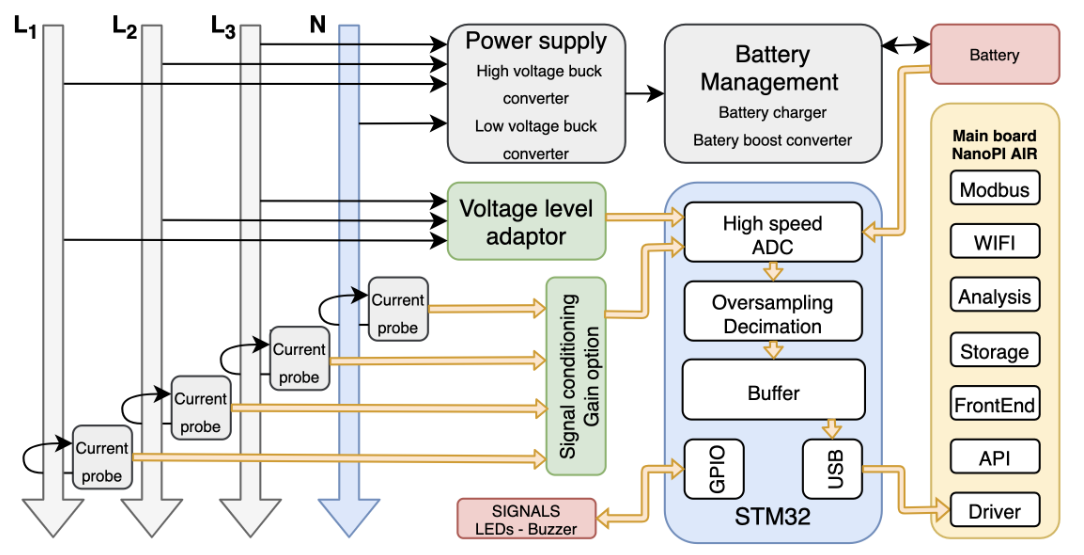
\includegraphics[width=0.8\textwidth]{figuras/openzmeter-diagrama.png}
    \fonte{CITAR Open Source Oz3.pdf}
\end{figure}

Para o multímetro, foi utilizado um diagrama de blocos disponível no site da (CITAÇÃO) \autoref{fig:ozm3flowchart} \textit{Texas Instruments}, que explica o funcionamento de um produto completo.

\begin{figure}[h]%% Ambiente figure
    %\captionsetup{width=0.55\textwidth}%% Largura da legenda
    \caption{Exemplo de um Diagrama de Blocos de um Multímetro}%% Legenda
    \label{fig:multimeterflowchart}%% Rótulo
    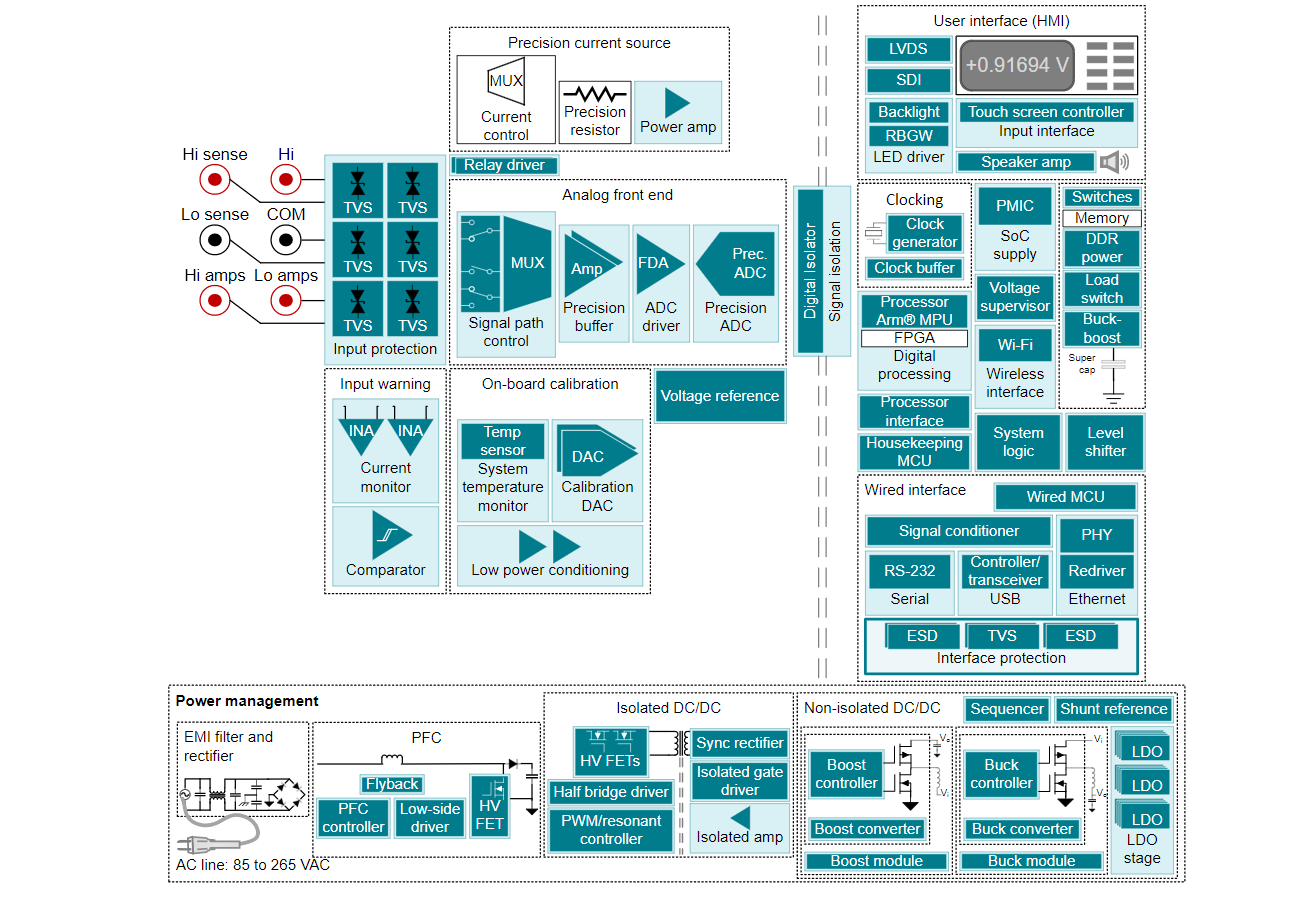
\includegraphics[width=1\textwidth]{flowchart}%% Dimensões e localização
    \fonte{Texas Instruments}%% Fonte
\end{figure}

% RAFAEL --------------------------------------------------------------------------------------------------------


\section{Proteção de Entrada}\label{sec:InputProtection}

Proteção de entrada é um assunto extremamente abrangente quando se trata de circuitos eletrônicos. Dependendo da função que este tenha que exercer, existem infinitas topografias que podem ser consideradas. Algumas exigências, porém, são comuns, como a necessidade de um circuito de proteção contra descargas eletrostáticas, ou ESD (Electrostatic Discharge). Tais descargas podem entregar picos de tensão extremamente altos, chegando até a 30 kV, o que é extremamente danoso a qualquer circuito que use semicondutores. Pulsos de pico tão alto quanto 2500 V já são o suficiente para danificar a maioria dos circuitos eletrônicos. Notóriamente, seres humanos são capazes de entregar descargas de até 20 kV porcausa da capacitância inata à sua fisiologia %%citar o documento http://www.reallyreallyrandom.com/zener/media/Zener_Theory_and_Design.pdf, página 65

    \subsection{ESD}\label{subsec:electrostaticDischarge}
    Esse tipo de proteção é necessária para circuitos que fazem interface com o meio físico e normalmente é exercida por um circuito básico de componentes TVS (Transient Voltage Supressor). Os semicondutores mais simples (e também regularmente) utilizados para exercer esta função são diodos Zener.
    
    Ao serem submetidos a uma tensão maior que à especificada como limite de operação do circuito a ser protegido, diodos Zener apresentam uma resistencia baixissima, fechando a passagem de corrente entre o circuito e o ground do equipamento. Este circuito pode apresentar uma configuração unidirecional ou bidirecional, dependendo da necessidade do circuito a ser protegido. 
    
    As \ref{fig:tvsUnidirecional} e \ref{fig:tvsBidirecional} demonstram a utilização basica de tal circuito e o conceito por trás da tensão de ruptura de tal semicondutor.

    \begin{figure}[h]%% Ambiente figure
        %\captionsetup{width=0.55\textwidth}%% Largura da legenda
        \caption{Exemplo de uso TVS Unidirecional}%% Legenda
        \label{fig:tvsUnidirecional}%% Rótulo
        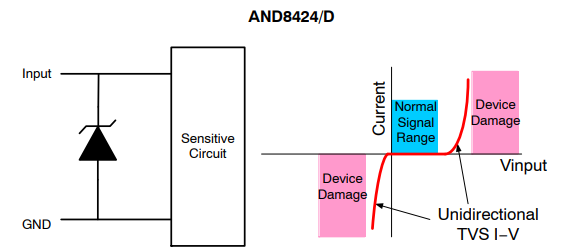
\includegraphics[scale=0.8]{tvs-unidirectional}%% Dimensões e localização
        \fonte{Adaptado de https://www.mouser.com/pdfdocs/AND8424-D.PDF, acesso em: 16/05/2023}%% Fonte
    \end{figure}

    \begin{figure}[h]%% Ambiente figure
        %\captionsetup{width=0.55\textwidth}%% Largura da legenda
        \caption{Exemplo de uso TVS Bidirecional}%% Legenda
        \label{fig:tvsBidirecional}%% Rótulo
        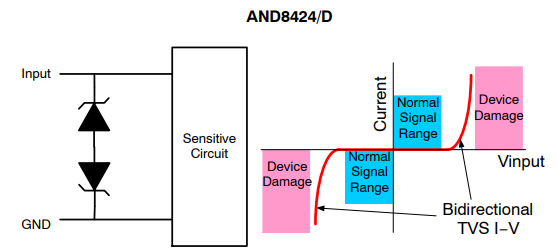
\includegraphics[scale=0.8]{tvs-bidirectional}%% Dimensões e localização
        \fonte{Adaptado de https://www.mouser.com/pdfdocs/AND8424-D.PDF, acesso em: 16/05/2023}%% Fonte
    \end{figure}

    \subsection{Proteção Específica para Equipamentos de Medição de Sinais Elétricos}\label{subsec:especProtec}

    Primeiramente, se põe necessário explicar sobre a classificação de proteção quando se fala de equipamentos elétricos. A classificação mais robustamente utilizada é a CAT, que vai de CAT I a CAT IV. Os numerais indicam o potencial de energia que o sistema pode entregar caso ocorra um curto-circuito ou um transiente de tensão, então um instrumento CAT III tem que estar protegido contra transientes muito maiores que um dispositivo CAT II. 

    Dispositivos CAT IV devem estar protegidos a nivel de distribuição de energia, pois estes serão utilizados em conexão entrada de energia de uma facilidade. Dispositivos CAT III devem estar protegidos a nivel de distribuição interna (quadros de distribuição), podendo esta ser trifásica ou monofásica. Dispositivos CAT II devem estar protegidos a nivel de equipamento terminal ou de uso comum, sendo estes eletrodomésticos e afins. Dispositivos CAT I devem estar protegidos a nivel de circuitos eletronicos e transformadores de baixa potência. %%ref: https://www.ecmweb.com/test-measurement/article/21247639/understanding-the-cat-rating-system

    \begin{figure}[htb]%% Ambiente figure
        %\captionsetup{width=0.55\textwidth}%% Largura da legenda
        \caption{Ilustração da Classificação CAT}%% Legenda
        \label{fig:CATrating}%% Rótulo
        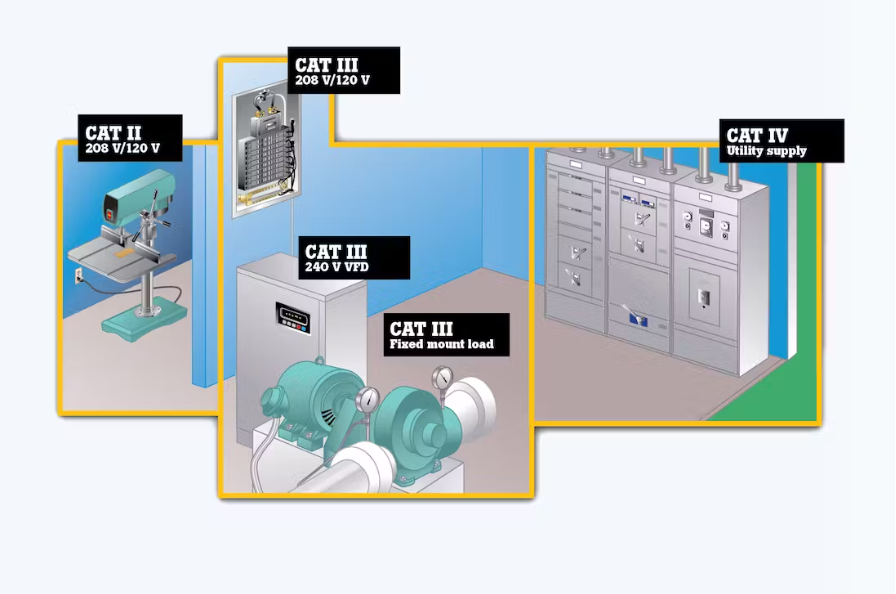
\includegraphics[scale=0.6]{CATrating}%% Dimensões e localização
        \fonte{Adaptado de https://www.ecmweb.com/test-measurement/article/21247639/understanding-the-cat-rating-system, acesso em: 17/05/2023}%% Fonte
    \end{figure}


    
        \subsubsection{Proteção de Entrada para Circuitos de Corrente}\label{subsec:protecaoCorrente}

        O circuito de proteção para o input de correntes se divide em duas partes, sendo uma delas para o range de A (Amperes) e os ranges de mA e µA.

	    Para o input de Amperes, é utilizado um fusível HRC (High Rupturing Capacity), geralmente de 11 A e 1000 V, para se prevenir arcos voltaicos após a queima do fusível, negando a possibilidade de uma continuação da condução de curto-circuito ou sobrecorrente. Logo após, é conectado um shunt de quatro terminais, 0R005 $\Omega$, entre o ground e o input, no qual será feita a medida.

	    Para o input de mA e µA, também é utilizado um fusível HRC, mas de 500 mA e 1000 V. Em sequência, é colocado um retificador em ponte de diodos entre o canal e o ground, para dar clamp em possíveis sobretensões (normalmente ocasionada pela utilização errônea do equipamento, colocando-se o input de corrente para medir tensão) até que o fusível possa atuar. Internamente, há um switch entre mA e µA. 

        Para o switch de mA, é contectado em série um resistor shunt de 4R995 $\Omega$ com o shunt do range de A (0R005 $\Omega$), para ser feita a medição em uma resistência total de 5 $\Omega$.

        Para o switch de µA, é conectado um resistor shunt de 500 $\Omega$, no qual será feita a medição. %%ref: https://lygte-info.dk/info/DMMDesignProtection%20UK.html

        \subsubsection{Proteção de Entrada para Circuitos de Tensão}\label{subsec:protecaoTensao}

        O circuito de proteção para o input de tensão é simples, sendo este composto de um resistor WW (WireWound) em série com um termistor PTC (Positive Temperature Coefficient) em série com um resistor de 10 M$\Omega$, no qual será feita a medida. 

        Conectado em paralelo ao resistor de 10 M$\Omega$ com o ground input, há uma série de varistores MOV (Metal Oxide Varistor) de rápida atuação como proteção para transientes de sobretensão, até que o termistor consiga esquentar. Pode ser utilizado somente um varistor, mas uma série destes aumenta a distância de fuga de corrente, reduzindo a chance de arcos voltaicos e também dissipando energia entre vários componentes, melhorando a proteção.

        Uma parte importante do design geral da PCB (Printed Circuit Board) são slots de isolamento de alta tensão, que se resumem a espaços abertos entre partes da placa, que vão receber altas tensões em funcionamento indesejado, para minimizar as chances de arcos voltaicos entre partes do circuito, como explícito na \ref{fig:exemploPCB}. %%ref: https://lygte-info.dk/info/DMMDesignProtection%20UK.html

        \begin{figure}[h]%% Ambiente figure
            %\captionsetup{width=0.55\textwidth}%% Largura da legenda
            \caption{Fluke 28-II PCB}%% Legenda
            \label{fig:exemploPCB}%% Rótulo
            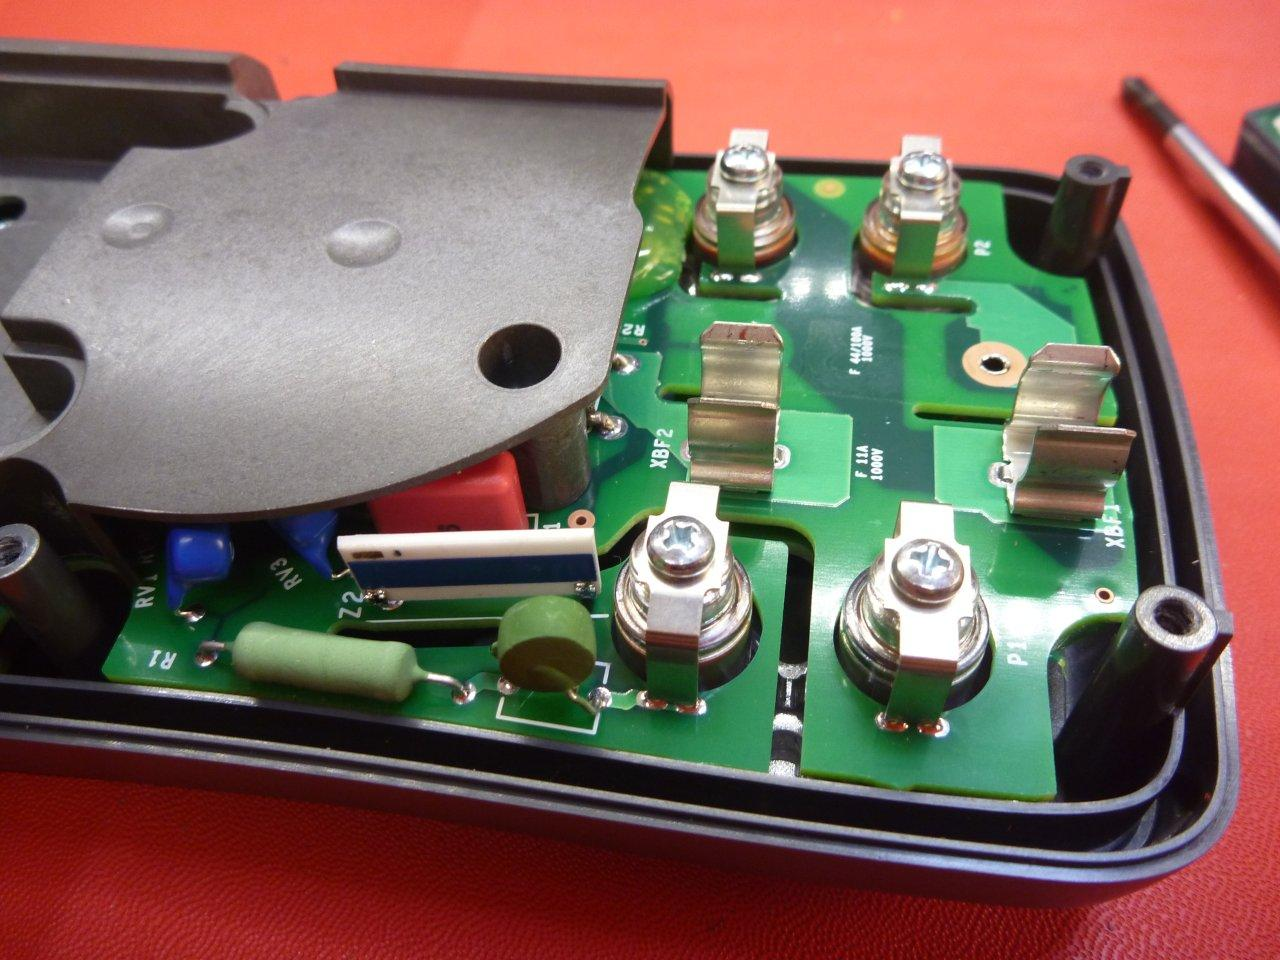
\includegraphics[scale=0.6]{divetPCB}%% Dimensões e localização
            \fonte{Adaptado de https://www.mjlorton.com/forum/index.php?topic=150.0, acesso em: 17/05/2023}%% Fonte
        \end{figure}    








\section{Calibração}\label{sec:OpenLoopCalibration}

\section{Referência de Tensão}\label{sec:VoltageReference}

\section{Conversor Analógico Digital}\label{sec:ADC}

\subsection{Condicionamento de Sinal}\label{sec:SignalConditioning}


% ANDREY------------------------------------------------------------------------

\section{Aquisição de Sinal}\label{sec:aqSignal}

    \subsection{Monofásica e Monocanal}\label{subsec:aqSMono}

    \subsection{Trifásica e Multicanal}\label{subsec:aqSMulti}
        \subsubsection{Resistor Shunt}\label{subsubsec:resiShunt}
Neste tipo de medição, um resistor de valor extremamente baixo (< 0,1 Ohm) é colocado em série com o circuito no qual se deseja medir a corrente elétrica, quando esta atravessa o componente, ocorre uma queda de tensão proporcional. Essa queda de tensão pode ser então medida diretamente através de um ADC ou amplificada e então medida para se obter os valores da corrente original. [Current Sensing Technniques]
Para a aplicação do multimedidor de 3 canais independentes de corrente, torna-se necessária algum tipo de isolação. Isso pode ser obtido utilizando-se de amplificadores isoladores neste caso – amplificadores operacionais que possuem duas referências isoladas entre si, permitindo uma medição da queda de tensão sobre o resistor shunt para cada canal sem interferência mútua, como exemplo o AD202 na \ref{AD202}.

\begin{figure}[h]
    \caption{AD202 um exemplo de amplificador isolador}
    \label{AD202}
    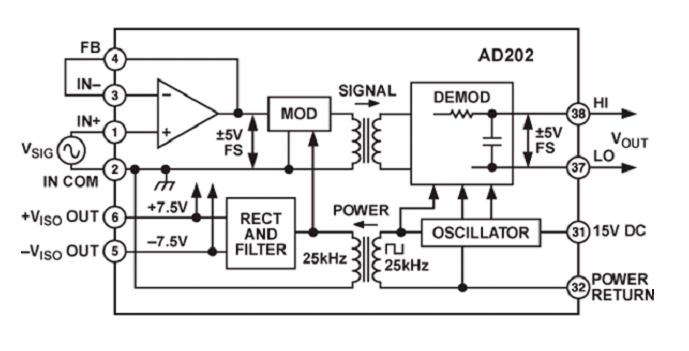
\includegraphics[width=0.8\textwidth]{figuras/AD202-ampop-isolado.png}
    \fonte{CITAR DATASHEET AD202}
\end{figure}

Esse tipo de amplificador, porém, apresenta alto custo e possui uma variação de leitura considerável com a temperatura. São inferiores em precisão a outros métodos de medição que realizam o isolamento do circuito inerentemente por seus aspectos construtivos. 

\subsubsection{Bobina Rogowski}\label{subsubsec:Rogowski}

Utilizando-se do princípio da Lei da Indução de Faraday, a bobina Rogowski trata-se de um loop fechado de fio enrolado em volta de um aro. Esse aro envolve o condutor que, por sua variação de corrente, induz uma tensão elétrica proporcional ao número de espiras e a intensidade da própria corrente a ser medida. Para a medida dos valores obtidos pela bobina Rogowski, é necessário o uso de um integrador (por vezes acoplado no próprio cabo da ponteira de medição) para relacionar a derivada da corrente com a tensão obtida em seus terminais, podendo causar certo erro introduzido pela operação.

\begin{figure}[h]
    \caption{Bobina Rogowski aberta}
    \label{fig:rogowski-bobina}
    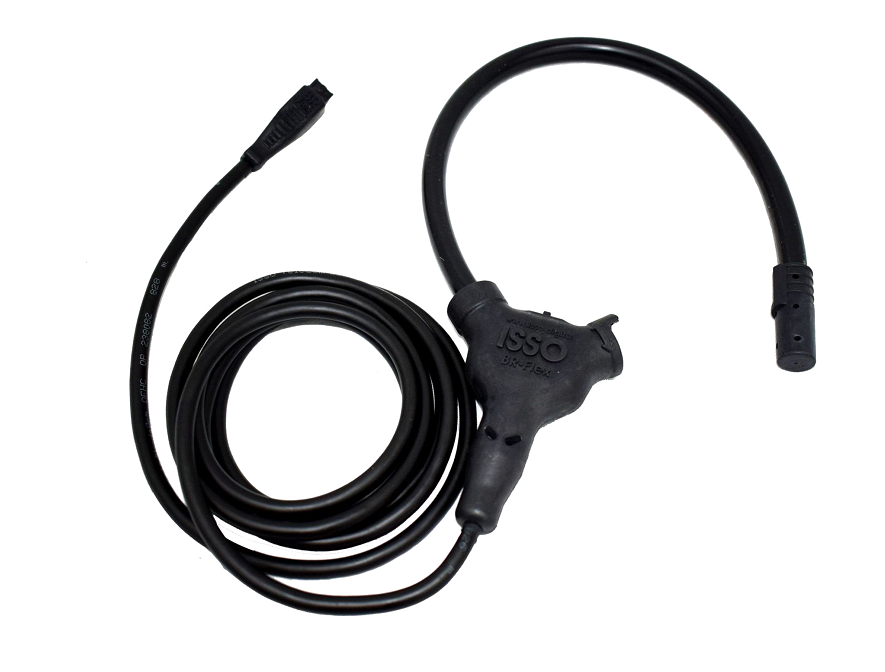
\includegraphics[width=0.8\textwidth]{figuras/bobina-rogowski.png}
    \fonte{CITAR Metodos de medição (artigo)}
\end{figure}

É um método amplamente utilizado para medições de altas correntes e suporta uma grande faixa de frequências. Tem um custo próximo dos transformadores de corrente e insere menos impedância parasita no circuito. [CITAR Current Sensing Techniques]

\subsubsection{Transformador de Corrente}\label{subsubsec:t-corrente}

O princípio de funcionamento do transformador de corrente é parecido com o da bobina Rogowski: possui um primário e um secundário com uma razão de voltas que permite que a tensão induzida seja lida em sua saída. A diferença deste para a bobina Rogowski é que existe agora um núcleo com certa permeabilidade magnética e o secundário possui um resistor Rs que permite uma medição mais simplificada da corrente de entrada.
Nesse tipo de medição, a própria saída do transformador de corrente é proporcional a entrada de corrente, não sendo necessário um integrador como é o caso da bobina Rogowski. Devido a sua construção, seu sinal de saída também não necessita de nenhum tipo de amplificação, podendo ser lido diretamente por um ADC. É teoricamente impossível medir correntes contínuas com esse método, porém, caso seja possível pulsar essa corrente, utilizando um circuito acessório de desmagnetização e, respeitando os tempos necessários entre os pulsos, é possível obter uma medida satisfatória.

\begin{figure}[h]
    \caption{Circuito completo com transformador de pulso para medição CA/CC}
    \label{fig:circuito-tc-dc}
    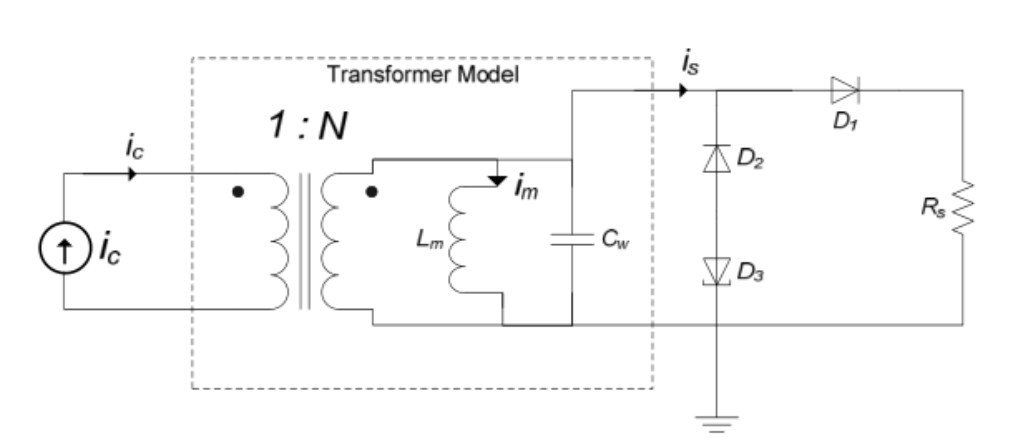
\includegraphics[width=0.8\textwidth]{figuras/transform-corrente-dc.png}
    \fonte{CITAR Metodos de medição corrente (artigo)}
\end{figure}

\subsubsection{Circuito Integrado de Medição \textit{(hall effect)}}\label{subsubsec:halleffect}

Existem circuitos integrados capazes de medir a corrente alternada de maneira isolada do
restante do circuito. Utilizando-se do efeito hall, o campo magnético gerado pela corrente
que passa entre seus terminais é medida por um sensor montado diretamente no substrato
do chip. Uma tensão proporcional a esse campo é fornecida pelo CI como saída e pode ser
medida por um ADC, recuperando-se o valor da corrente original.
O uso dessa tecnologia traz custo baixo em relação ao uso de TC's ou bobinas Rugowski,
fácil implementação no sistema, isolamento diretamente no chip.
Tal medição, porém, possui uma resolução de cerca de 100 mV/A (considerando um CI que
suporte acima de 10 A) e um ruído intrínseco de 11 mV.[CITAR DATASHEET ACS712]

\section{Aviso de Entrada Incorreta \textit{(Input Warning)}}\label{sec:inpWarning}

    \subsection{Monofásico e Monocanal}\label{subsec:inpWMono}

    \subsection{Trifásico e Multicanal}\label{subsec:inpWMulti}

\section{Isolador de sinal digital \textit{(Digital Signal Isolator)}}\label{sec:DSIsolator}

\section{MCU e Interface de Comunição}\label{sec:MCUInterface}

    \subsection{Microcontroladores}\label{subsec:MCU}

    \subsection{Interface de Comunicação}\label{sec:Interface}